\documentclass[12pt]{amsart}
\usepackage[margin=1in]{geometry}
\usepackage{hyperref}
\usepackage{natbib}
\usepackage{times}
\usepackage{amsfonts}
\usepackage{amsmath}
\usepackage[psamsfonts]{amssymb}
\usepackage{amstext}
\usepackage{amsthm}
\usepackage{latexsym}
\usepackage{color}
\usepackage{graphicx}
\usepackage{subfig}
\usepackage{enumerate}
\usepackage{enumitem}
\usepackage{url}
\usepackage{comment}
\usepackage{multirow}
\usepackage{hhline}

\makeatletter
\newtheorem*{rep@theorem}{\rep@title}
\newcommand{\newreptheorem}[2]{%
\newenvironment{rep#1}[1]{%
 \def\rep@title{#2 \ref{##1}}%
 \begin{rep@theorem}}%
 {\end{rep@theorem}}}
\makeatother

\hypersetup{
  colorlinks   = true,
  urlcolor     = blue,
  linkcolor    = blue,
  citecolor   = blue
}

\let\Pr\undefined
\def\Rset{\mathbb{R}}
\def\Nset{\mathbb{N}}
\def\vcdim{\text{VCdim}}
\def\pdim{\text{Pdim}}
\DeclareMathOperator*{\E}{\mathbb{E}}
\DeclareMathOperator*{\Pr}{\mathbb{P}}
\DeclareMathOperator*{\argmax}{\rm argmax}
\DeclareMathOperator*{\argmin}{\rm argmin}
\DeclareMathOperator{\sgn}{sgn}
\DeclareMathOperator{\sign}{sign}
\DeclareMathOperator{\supp}{supp}
\DeclareMathOperator{\range}{range}
\DeclareMathOperator{\rank}{rank}
\DeclareMathOperator{\diag}{diag}
\DeclareMathOperator{\Tr}{Tr}
\providecommand{\norm}[1]{\| #1 \|}
\providecommand{\frobp}[2]{\langle#1, #2\rangle_F}
\def\dqed{\relax\tag*{\qed}}

\newcommand{\set}[1]{\{#1\}}
\newcommand{\iprod}[2]{\left\langle #1, #2 \right\rangle}
\newcommand{\h}{\widehat}
\newcommand{\tl}{\widetilde}
\newcommand{\Alpha}{{\boldsymbol \alpha}}
\newcommand{\mat}[1]{{\mathbf #1}}
\newcommand{\be}{\mat{e}}
\newcommand{\bu}{\mat{u}}
\newcommand{\bh}{\mat{h}}
\newcommand{\n}{\mat{n}}
\newcommand{\K}{\mat{K}}
\newcommand{\N}{\mat{N}}
\newcommand{\0}{\mat{0}}
\newcommand{\w}{\mat{w}}
\newcommand{\x}{\mat{x}}
\newcommand{\cB}{\mathcal{B}}
\newcommand{\cL}{\mathcal{L}}
\newcommand{\cX}{\mathcal{X}}
\newcommand{\Ind}{\mathds{1}}
\newcommand{\1}{\mathds{1}}
\newcommand{\R}{\mathfrak{R}}
\newcommand{\e}{\epsilon}
\newcommand{\EQ}{\gets}
\newcommand{\wt}{\widetilde}
\newcommand{\ssigma}{{\boldsymbol \sigma}}
\newcommand{\tts}{\tt \small}
\newcommand{\TO}{\mbox{ {\bf to }}}

\newtheorem{theorem}{Theorem}
\newreptheorem{theorem}{Theorem}
\newtheorem{lemma}[theorem]{Lemma}
\newreptheorem{lemma}{Lemma}
\newtheorem{definition}[theorem]{Definition}
\newtheorem{corollary}[theorem]{Corollary}
\newreptheorem{corollary}{Corollary}
\newtheorem{proposition}[theorem]{Proposition}
\newreptheorem{proposition}{Proposition}

\newenvironment{code}{\begin{tabbing}
    12\=12\=12\=12\=12\=12\=12\=12\= \kill }
  {\end{tabbing}}
\newcommand{\ignore}[1]{}


\title{WikiNet: Wikipedia as a Network}
\author{Chen Zhang (cz1389) \& Guang Yang (gy552)}

\begin{document}

\begin{abstract}
We present the prototype of WikiNet, a relation-based search engine for Wikipedia. A heuristic crawler is built to colloect a small propotion of wikipedia pages. Using the the structural infomation and content of the pages, we model the dataset as a directed weighted graph. Based on this graph, WikiNet carries our similarity based search. So far, two functions are implemented, namely, to search a page's most related pages, and to search the  most related path between a pair of pages. Analysis show that WikiNet provides much higher-quality relations between wikipedia pages than na\"ive BFS strategy. 
\end{abstract}

\maketitle

\section{Introduction}

Wikipedia is so far the largest public online database of knowledge. 
When searching over wikipedia, it is almost certain that there will be a page excatly match the query. 
Aside from the incredibly high precision, wikipedia also enjoys a high degree of diversity. The divsersity of wikipeda is reflected by the numerous hyperlinks to other wikipedia articles on any page. 
When reading wikipedia articles, people always follow the links to some other related topics(usually in a depth-first pattern). 
At the end of the day, we can be very far from what we intended in the first place. 

The quality of the relation between connected pages varies drasticly. If a link with poor relation is followed, people may be diverted into a very different field. 

That is where WikiNet starts. We seek to search for high quality relations in wikipedia. In general, we provide a new document scoring method for networked databases such as wikipedia. 
In Section~\ref{sec:wiki}, we introduce a heuristic crawler that help us collect reasonable amount of kind-of-related wikipedia pages. 
In Section~\ref{sec:net}, we modeled our datasets as directed weighted graphs based on the structural information and the content of the pages. 
In Section~\ref{sec:wikinet}, the features of WikiNet are introduced. Several experienments are presented. 
In Section~\ref{sec:eva}, we raised an evaluation measurement and discussive the performance of WikiNet against the na\"ive approach. 
We conclude in Section~\ref{sec:con}. 

\section{The Wiki part: Heuristic crawler}
\label{sec:wiki}
Because of our limited storage and computation resource, it is not feasible for us to traversd and index the whole wikipedia. As a result, heuristic methods are heavily used.

Wikipedia pages have in- and out-links to other pages. Some links are pointing at a highly related page, while others are not. (i.e. The page of \href{https://en.wikipedia.org/wiki/Apple}{apple} the fruit, has a hyper link to \href{https://en.wikipedia.org/wiki/Adam_and_Eve}{Adam and Eve}. However, the word of "apple" doesn't even appear on the latter. In fact, it is \href{https://en.wikipedia.org/wiki/Apple_(symbolism)}{apple} the symbol that is closely related to Adams and Eves. ) So when crawling wikipedia pages, we conduct for- and backwards evaluation and only index the highly related pages. 

\begin{figure}[htb]
\begin{code}
\textsc{HeuristicCrawler}($seed$, $maxDepth$): \\
\> \textsc{Queue} $U$ \\
\> \textsc{Set} $V$ \\
\> $U.\textsc{Push}(\langle seed, 0 \rangle)$ \\
\> \textbf{While} $U.\textsc{NotEmpty}()$: \\
\>\> $ \langle p, depth \rangle \leftarrow U.Pop()$ \\
\>\> \textbf{If} $p$ is closely related to its parent: \\
\>\>\> $V.\textsc{Insert}(p)$ \\
\>\> \textbf{If} $depth < maxDepth$: \\
\>\>\> \textbf{For all} $hyperlink$ in the content of $p$: \\
\>\>\>\> \textbf{If} $hyperlink$ is important in $p$: \\
\>\>\>\>\> $U.\textsc{Push}(\langle hyperlink, depth+1 \rangle)$\\ 
\> \textbf{Return} $V$
\end{code}
\caption{Heuristic crawler alogrithm}
\label{al:crawler}
\end{figure}

The algorithm of the heuristic crawller is shown as Fig.~\ref{al:crawler}. In order to guarantee that only the related pages are indexed, we perform forward and backward check. 

\begin{description}
\item[Forward] In order to judge if a $hyperlink$ is important in page $v$, we devloped a scoring mechanism. Each occurrence of the anchor text in the introduction part\footnote{The crawler may fail to recoginzed the introduction part for some pages. Chances are that the crawler may leave informative links. However those pages may be recovered somewhere wlse. } counts for $3$ point, while others count for $1$ point. $Hyperlinks$ that score \textbf{more than $1$ point} is considered realted. The related pages are added into the Queue
\item[Backward] The forward check guarantees that the page being visited is some how related to its parent. We perform a backward check to guarantee the mutual relation. Again, a scoring mechanism is introduced. Each link back to its parent page counts for $3$ points, and each reference to the title of its parent counts for $1$ point. Only the pages (except the seed) that scores \textbf{at least $3$ points} are indexed. If a page is found irrelevant, it is droped immediately along with the hyperlinks in it. 
\end{description}

This stragety is not perfect. For example, it is common sense that \href{https://en.wikipedia.org/wiki/Deep\_learning}{deep learning} has a lot to do with \href{https://en.wikipedia.org/wiki/Yann\_LeCun}{Yann LeCun}. However, the former wasn't mentioned in the content (literally, not a word) of the latter. In this case, when visiting \href{https://en.wikipedia.org/wiki/Yann\_LeCun}{Yann LeCun} and perform backward check, the page will be marked as irrelevant. Actually, the wikipedia page of  \href{https://en.wikipedia.org/wiki/Yann\_LeCun}{Yann LeCun} is of such a low quality that it is almost isolated. 

We limit the depth of the BFS crawling to $4$ and crawled pages from $4$ different seeds. A brief discription of the 

\begin{table}[htb]
\centering
\begin{tabular}{|l|r|r|}\hline
seed & \# visted pages & \# indexed pages \\ \hline
\href{https://en.wikipedia.org/wiki/Apple}{\textsf{https://en.wikipedia.org/wiki/Apple}} & 13956 & 6619 \\ \hline
\href{https://en.wikipedia.org/wiki/Apple\_Inc.}{\textsf{https://en.wikipedia.org/wiki/Apple\_Inc.}} & 14929 & 6050 \\ \hline
\href{https://en.wikipedia.org/wiki/Artificial\_intelligence}{\textsf{https://en.wikipedia.org/wiki/Artificial\_intelligence}} & 27123 & 12682 \\ \hline
\href{https://en.wikipedia.org/wiki/New\_York\_University}{\textsf{https://en.wikipedia.org/wiki/New\_York\_University}} & 17688 & 6769 \\ \hline 
\end{tabular}
\caption{A discription of the dataset we collected. }
\label{tbl:dataset}
\end{table}

We only conduct experiment on the two apples. You may search using the keyword "apple" to find out which one is currently running. 


\section{The Net part: Directed weighted graph}
\label{sec:net}
Now that Wikipedia is an online database, the system is by nature a complex network, where artibles are the nodes, and hyperlinks the edges. We build a graph from the dataset. We used TF-IDF to index the main content of the pages and marked the weight of the edges using the cosine coefficent between the two pages. We end up with a directed weighted graph. We visualized the graph resulted from 3 of the 4 datasets. 

\begin{figure}[htb]
\centering
\subfloat[\href{https://en.wikipedia.org/wiki/Apple}{apple}]{
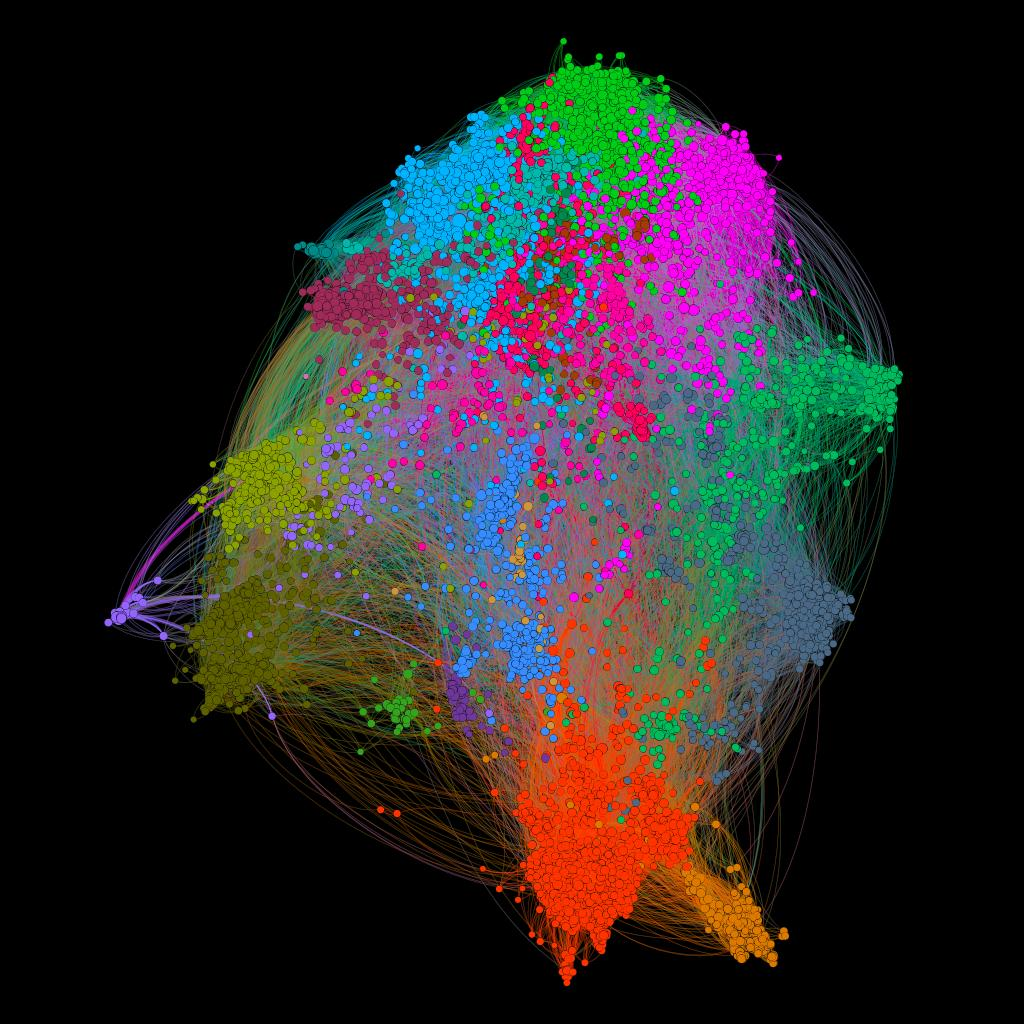
\includegraphics[height=2in]{apple}
\label{fig:net.apple}
}
~
\subfloat[\href{https://en.wikipedia.org/wiki/Apple_Inc.}{Apple Inc.}]{
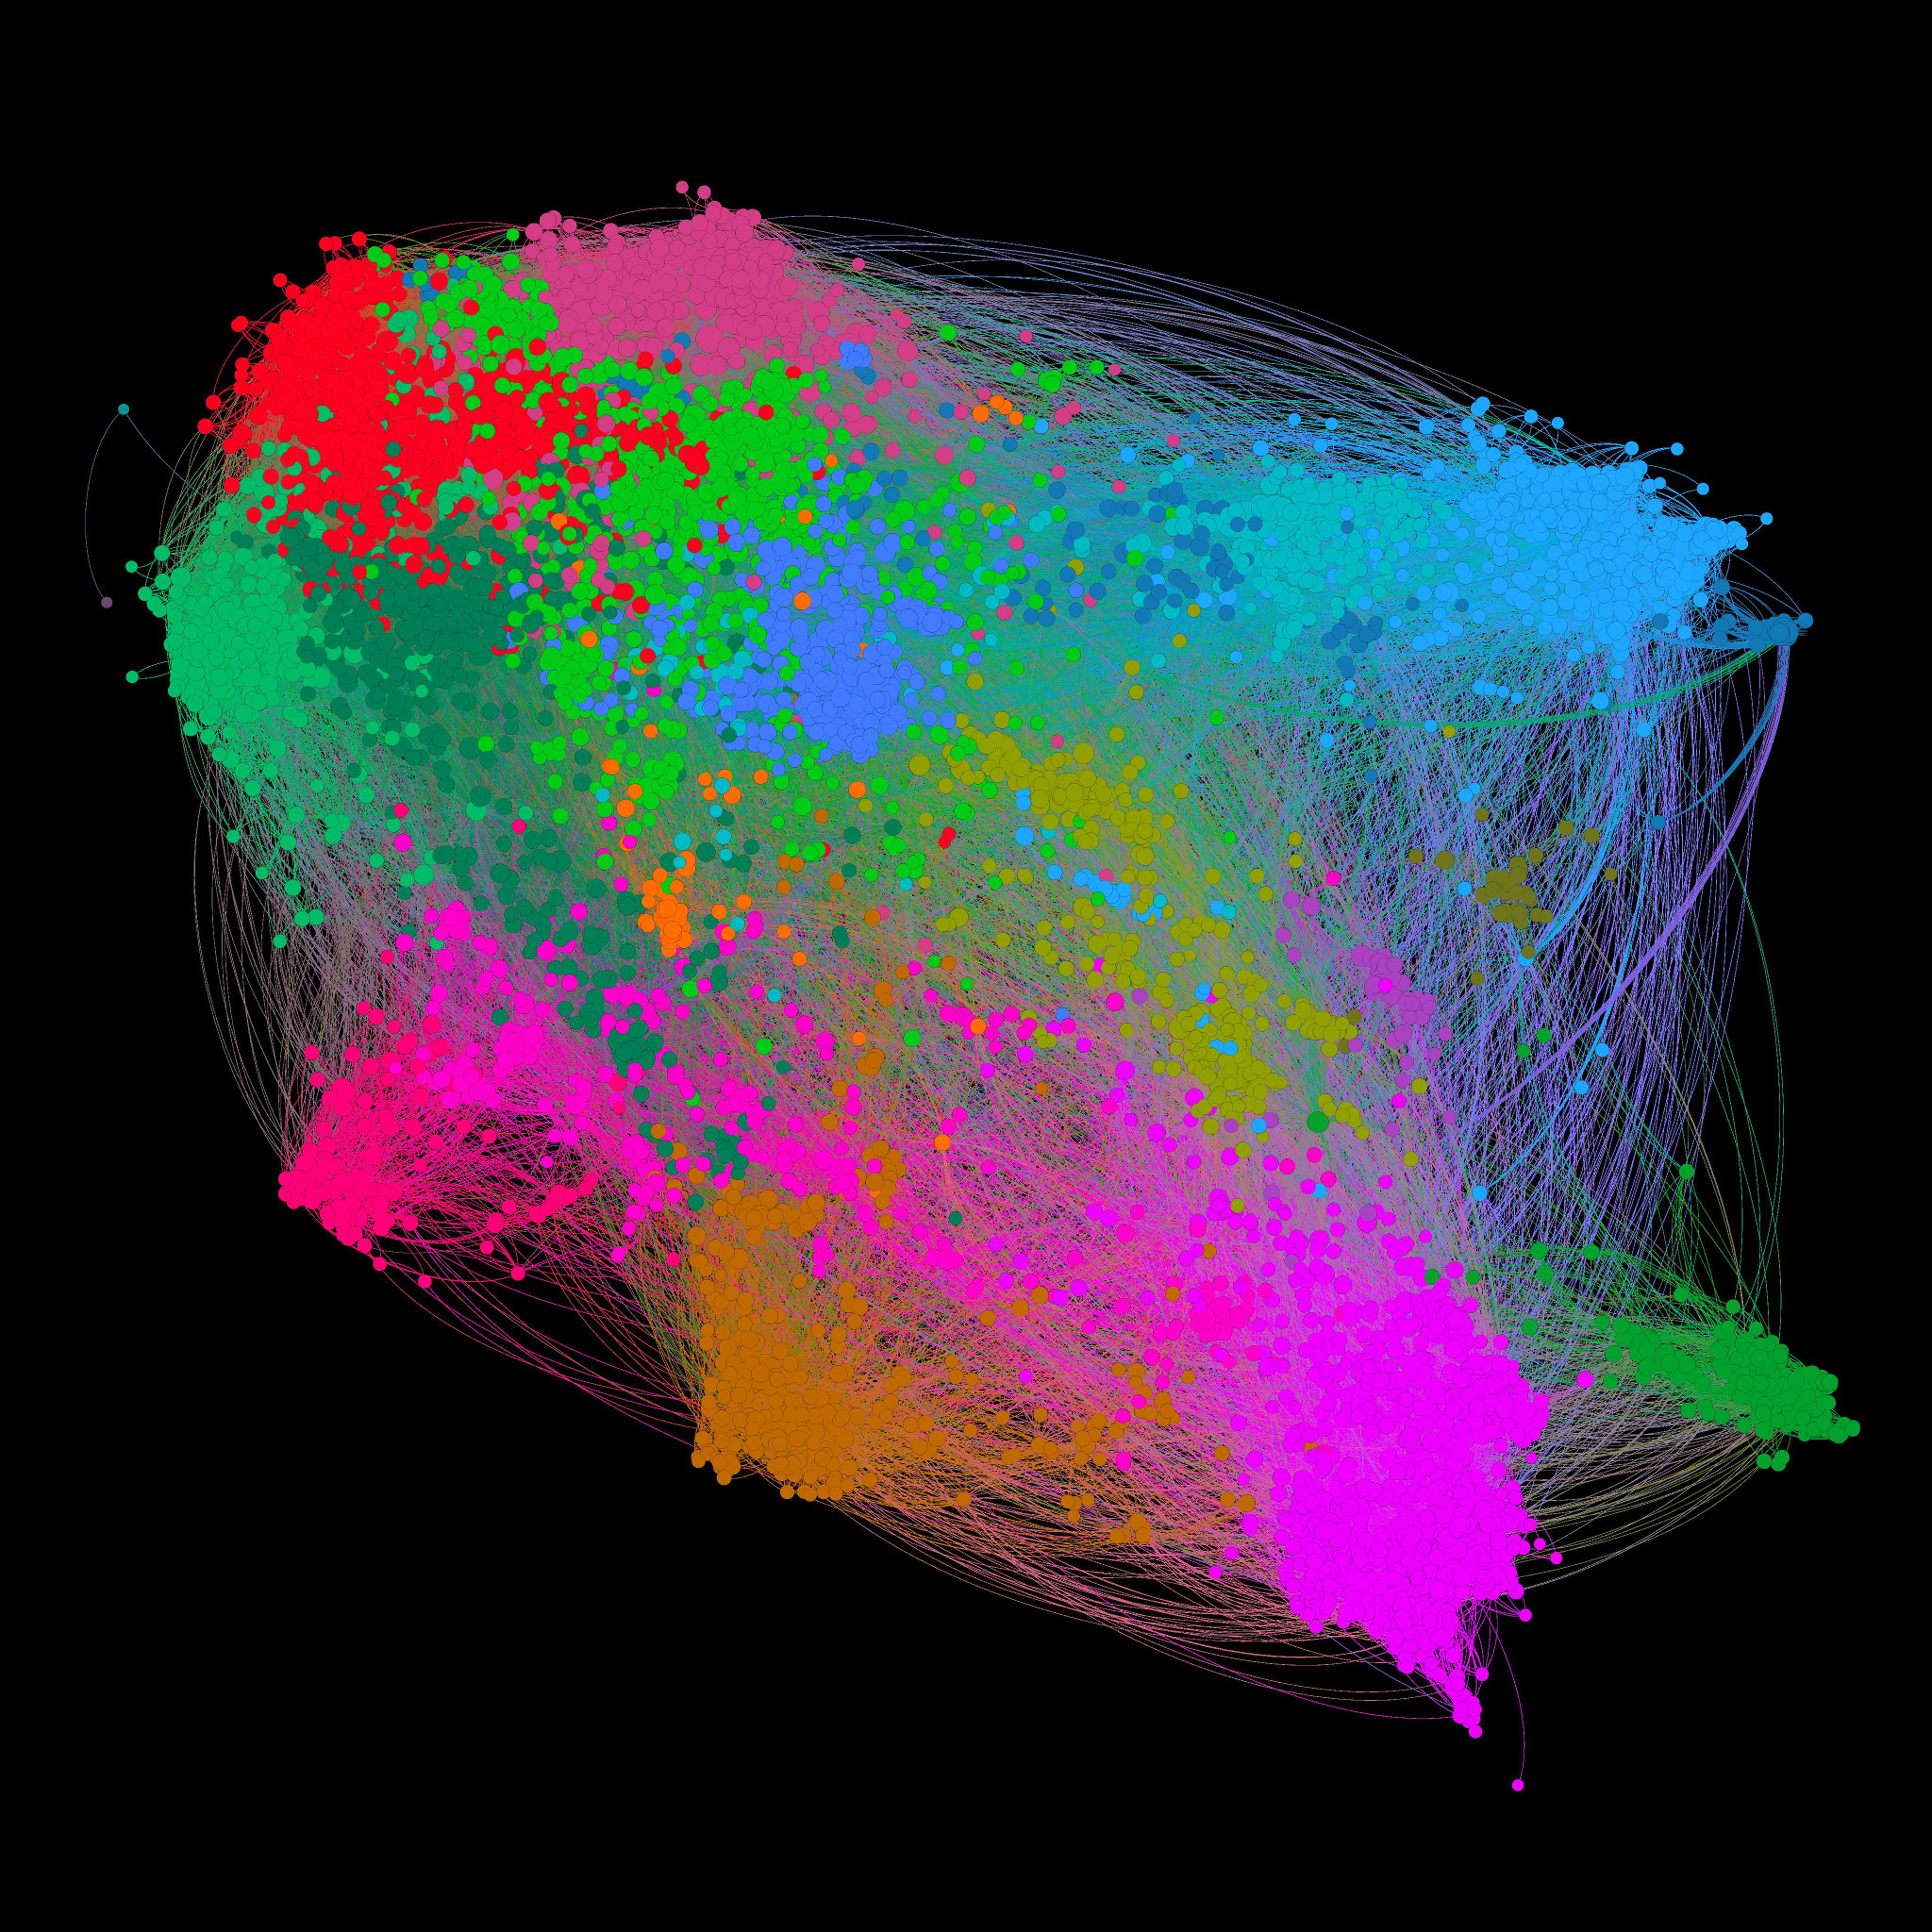
\includegraphics[height=2in]{inc}
\label{fig:net.inc}
}
~
\subfloat[\href{https://en.wikipedia.org/wiki/Artificial\_intelligence}{Artificial\_intelligence}]{
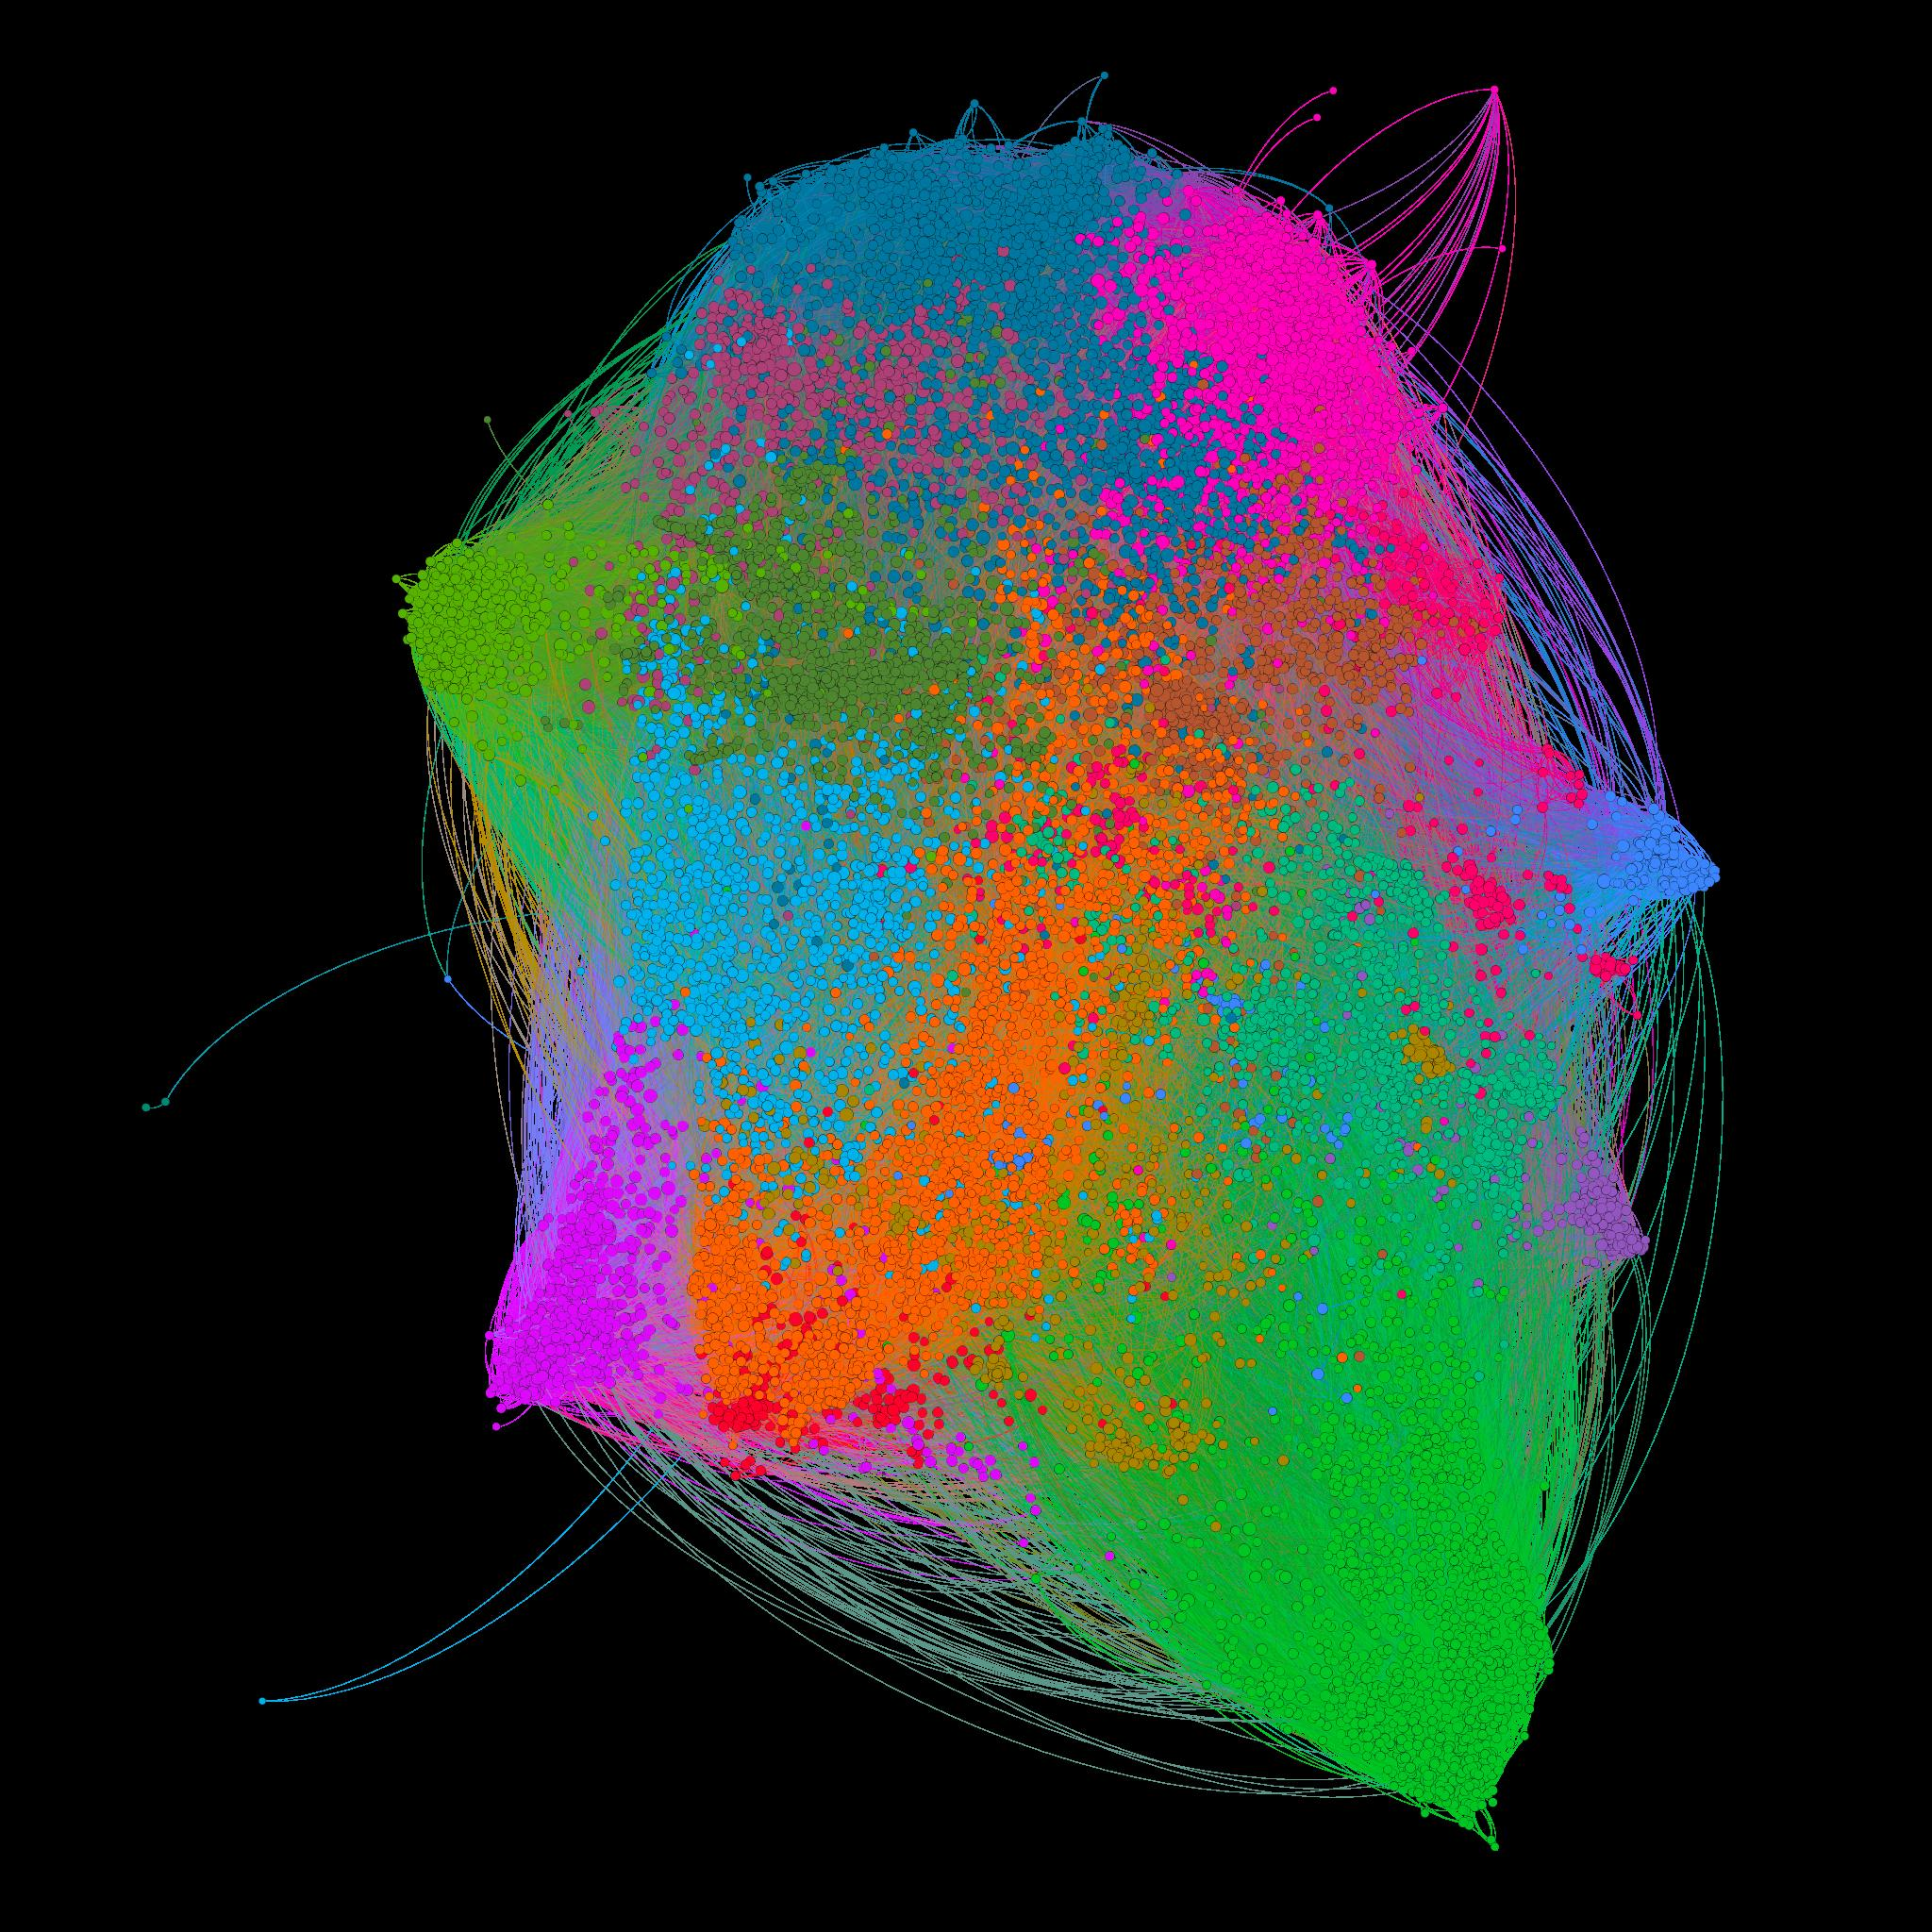
\includegraphics[height=2in]{ai}
\label{fig:net.ai}
}
\caption{An illustration of the graphs corresponding to the 3 of the datasets. Nodes of the same color fall into the same cluster based on a modularity-based community detection algorithm (the Louvain method \cite{blondel2008fast}).}
\label{fig:net}
\end{figure}

Finding the most related page or path is similar to the Longest Simple Path problem, which is NP-hard. Luckily, in our case, the weight of the edges are between 0 and 1. If we define the weight of a path as the  multiplication of the cosine coefficent of consecutive pair of pages on the path, 
\[
W(\mathcal{S}) = \prod_{i = 0}^{length(\mathcal{S})}w_{i, i+1}, \hbox{ where } \mathcal{S}=\langle v_0, v_1, \dots, v_{length(\mathcal{S})} \rangle, 
\]
which is a reasonable definition, the weight of a path decreases monotonously as we traverse the graph. This definition of the weight excludes loop in the path by definition. In this case, a smart modification to the widely-used all pair shortest path algorithm is sufficient to solve our problem. We therefore define the closeness between a pair of pages as the largest weight of all paths between them.
\[
D(v_i,v_j) = \max_{\mathcal{S} \in \{\langle v_i, \dots, v_j \rangle \}} W(\mathcal{S}) 
\]
The algorithm to solve the problem is given in Fig~\ref{al:dist}. It is based on the Floyd-Warshall algorithm. 
\begin{figure}
\begin{code}
\textsc{MostRelatedPath}$(cosineCoefficient)$: \\
\> $D = cosineCoefficient$ \\
\> $N=D.\textsc{size}$ \\
\> $M = \big[ M_{i,i} =i \big], i\in\{1,\dots,N\}]$ \\
\> \textbf{For} $ k \leftarrow 1,\dots, N$ : \\
\>\> \textbf{For} $ i \leftarrow 1,\dots, N$ : \\
\>\>\> \textbf{For} $ j \leftarrow 1,\dots, N$ : \\
\>\>\>\> \textbf{If} $D_{i,j} < D_{i,k} \times D_{k,j} $: \\
\>\>\>\>\> $D_{i,j} \leftarrow D_{i,k} \times D_{k,j}$ \\
\>\>\>\>\> $M_{i,j} \leftarrow k $ \\
\> \textbf{Return} $D,M$
\end{code}
\caption{Algorithm for all-pair most related path based on Floyd-Warshall}
\label{al:dist}
\end{figure}


\section{The WikiNet}
\label{sec:wikinet}
\subsection{How it works}

WikiNet is a relation-based search engine for wikipedia, where the records are too finely ground to tolerate any ambigurity, where diversity is implemented through the links between related articles. 
WikiNet makes uses of both the structure of wikipedia, and the content of it to carry out searching for relation among wikipedia pages. 

So far, we provide two search functions. 
\begin{enumerate}[label=\arabic*.]
\item Match the keywords with the most related wikipedia page in our dataset, then list the top 20 most related children pages (following out-links) and the top 20 most related parent pages (following in-links).
\item Take a pair of keywords. Match them with the most related wikipedia page in our dataset respectively. Then return the most related path bewteen the two pages. 
\end{enumerate}
The matching is done by firstly match the keywords with the titiles in the dataset. If no match is found, then the keywords are matched with the content. If nothing is archived, then a default page (very likely the seed) is matched. 

For example, in the apple\_inc dataset, the keyword of ``stanford'' will be matched with \href{https://en.wikipedia.org/wiki/Stanford,\_California}{Stanford, California} (the word of ``california'' may have a smaller score than ``university'', so \href{https://en.wikipedia.org/wiki/Stanford\_University}{Stanford University} ranks lower). However, the keyword of ``yann lecun'' will be matched with \href{https://en.wikipedia.org/wiki/Deep\_learning}{deep learning}, because \href{https://en.wikipedia.org/wiki/Yann\_LeCun}{Yann LeCun} is not indexed in the data base. 

\subsection{Experiments}
\begin{description}
\item[Query] apple
\item[Matched Page] Apple\_Inc
\item[Related pages (out-links)] Apple III, Apple Store (retail), Apple Store, Apple TV, Apple II series, Macintosh, Apple Maps, Apple Watch, Apple Music, Apple I, ITunes Radio, Disk II, {\color{red}{Apple Inc.}}, TvOS, Macworld Conference \%26 Expo, Macworld/iWorld, IPhone, Steve Jobs, MacOS, IPhone 5 
\item[Related pages following in-links] IOS 6, ITunes, IOS, IPhone OS, IOS (Apple), IOS 5, IOS 5.1, IOS 7, IPod Shuffle, MacBook (Retina), ITunes Store, IOS 4, IOS 9, IBooks Author, System 6, IOS 8, IOS 10, IPod touch (fifth generation), IPod Touch, Apple Maps
\end{description}

From the above experiment shows the result if we search from the seed. The ``Apple\_Inc.'' in red is the same page as the source ``Apple\_Inc''. Because we didn't do duplication prevention, it forms a loop via some other pages. For a large company like Apple, Google, Facebook since they have many products, it is more likely that the popular and discussed ones appear in the out-link part, and the less popular or discussed ones show up in the in-link part. 

\begin{description}
\item[Query] uber
\item[Matched Page] Uber (company)
\item[Related pages (out-links)] San Francisco, Mobile app, Smartphone, Google, Criticism of Google, Google privacy, Google\%2B, San Francisco Bay Area, Portland Oregon, Google Search, Google Drive, Austin Texas, Google Maps API, Google Maps, San Jose California, San Bruno California, G Suite, Google Earth, Google Data Centers, Daly City 
\item[Related pages following in-links] Self-driving cars, Charlie Miller (security researcher), IOS 10, G Suite, San Francisco, San Francisco County, Apple Maps, Apple Inc, Apple Inc., Apple\_ Inc., Apple Computer, San Francisco Bay Area, IOS 9, Apple Pay, Google Drive, Google, Google Inc, Internet, Internet users, Google Docs  Sheets and Slides
\end{description}

From the second experiment, we get a sense that the out-link results are more about what the object is about, and the in-link results are more about what is the object. 



\begin{description}
\item[Query] ibm
\item[Matched Page] IBM 
\item[Related pages (out-links)] IBM PC, IBM Watson, Watson (artificial intelligence software), International Business Machines, IBM Personal Computer XT, PC DOS, IBM System x, Compaq Portable, IBM Personal System/2, BASICA, Personal computer, MS-DOS, Mainframe computer, The Weather Company, System/370, IBM PCjr, DOS, 86-DOS, Home computer, Industry Standard Architecture
\item[Related pages following in-links] IBM PC, IBM System i, {\color{red}IBM 1316, IBM 1405, IBM 355, IBM 1302, IBM 1301, IBM 3340, IBM 350}, Watson (artificial intelligence software), IBM Watson, IBM Power Systems, International Business Machines, IBM System 360 Model 91, IBM System/360 Model 91, IBM Personal System/2, System/360, PC DOS, IBM PC DOS, Compaq Portable
\end{description}

From the experiment with IBM, we can see that WikiNet suffers from duplication. {\color{red}IBM 1316, IBM 1405, IBM 355, IBM 1302, IBM 1301, IBM 3340} and {\color{red}IBM 350} are all redirected to \href{https://en.wikipedia.org/wiki/History_of_IBM_magnetic_disk_drives}{History of IBM magnetic disk drives}, which largely jeopardize the result to IBM-related query. 




\begin{description}
\item[Query] tesla
\item[Matched Page] Tesla Inc.
\item[Related pages (out-links)] Tesla Model S, Elon Musk, SolarCity, Neuralink, SpaceX, Zip2, Stanford Research Park, Solar energy, General Motors, OpenAI, Hyperloop, Falcon 9, Solar panel, SpaceX, Dragon, Sergey Brin, Smartphone, Larry Page, Falcon 1, Photovoltaic, Solar cell
\item[Related pages following in-links] Tesla Model S, Self-driving cars, Elon Musk, SolarCity, Neuralink, SpaceX, Solar power in the United States, Zip2, OpenAI, Hyperloop, Falcon 9, Solar power in Germany, Dragon spacecraft, SpaceX Dragon, Falcon 1, Photovoltaic, Photovoltaics, Sergey Brin, Renewable energy, Windows 10
\end{description}

Tesla Inc. in at depth $4$. The page is near the boarder of the graph, so there could be no enough pages for it to connect with. As a result, we see some unstatisfying results, such as windows 10, and some people having little to do with Tesla. However, we can notice that WikiNet is trying to provide high quality content (the solar power related results). 

\begin{description}
\item[Source] google
\item[Destination] tesla
\item[Source Page] Google
\item[Destination Page] Tesla Inc.
\item[Most Related Path] Google $\rightarrow$ Google Energy $\rightarrow$ SolarCity $\rightarrow$ Tesla Inc.
\end{description}

We can easily find a shorter path: Google $\rightarrow$ Larry Page $\rightarrow$ Tesla. But clearly WikiNet's answer gives a better sense. A better path should be involving AI-related topic. Unfortunately, we can not afford a dataset large enough to include all these pages. 

\section{Evaluation}
\label{sec:eva}
It is hard to evaluate a search engine. However, since WikiNet is working on the relation between wikipedia pages, we managed to figure out a reasonable measurement. 

For a source page, each page in the returned list several hops away (in the means of all-pair shortest path in a graph).  

Consider the na\"ive way of doing relation search. The most simple yet somehow reasonable way is to do na\"ive breadth-first search. In this case, in response to a query matched with page $q$, the na\"ive strategy will return a list of pages visited in a BFS fashion starting from the source page. 
In comparison, WikiNet returns the destinations of the 20 most related paths starting from the source. 

Denote the documents returned by the na\"ive strategy $ \mathcal{N}(q)=\{d_{q,i}\} $. Use $\mathcal{D}(d_{q,i})$  to mark the depth of document $d_i$ in the BFS tree rooted at $q$. Denote the list returned by WikiNet as $\mathcal{R}(q)=\langle r_{q,1},r_{q,2},\dots, r_{q,20}\rangle$

If we take the WikiNet result as a reference, the recall of the na\"ive stratergy can be represented as 
\[
Recall(q,k) = \frac{1}{\sigma(q,k)}
\huge|
\big[\bigcup_{i = 1}^{\sigma(q,k)} r_{q,i} \big]
\bigcap
\{ d_{q,j} \in \mathcal{N}(q) | \mathcal{D}(d_{q,j}) <= k \} 
\huge|,
\]
where $\sigma(q,k) = \min\{20,\big| \{ d_{q,j} \in \mathcal{N}(q) | \mathcal{D}(d_{q,j}) <= k \} \big|\}$, which means the number of pages within $k$ hops from $q$. The recall equation measures how many of the top $\sigma(q,k)$ pages are at most $k$ hops from $q$. 

We measured every of the $6050$ pages in the apple\_inc dataset. Since the dataset has only 4 layers, and we only return the top 20 pages, we consider $k\in \{1,2,3\}$ to be reasonalbe. 
We plot the CDF of $Recall(q,k): \forall q, \forall k \in \{1,2,3\}$ as Fig.~\ref{fig:cdf}. 
\begin{figure}[htb]
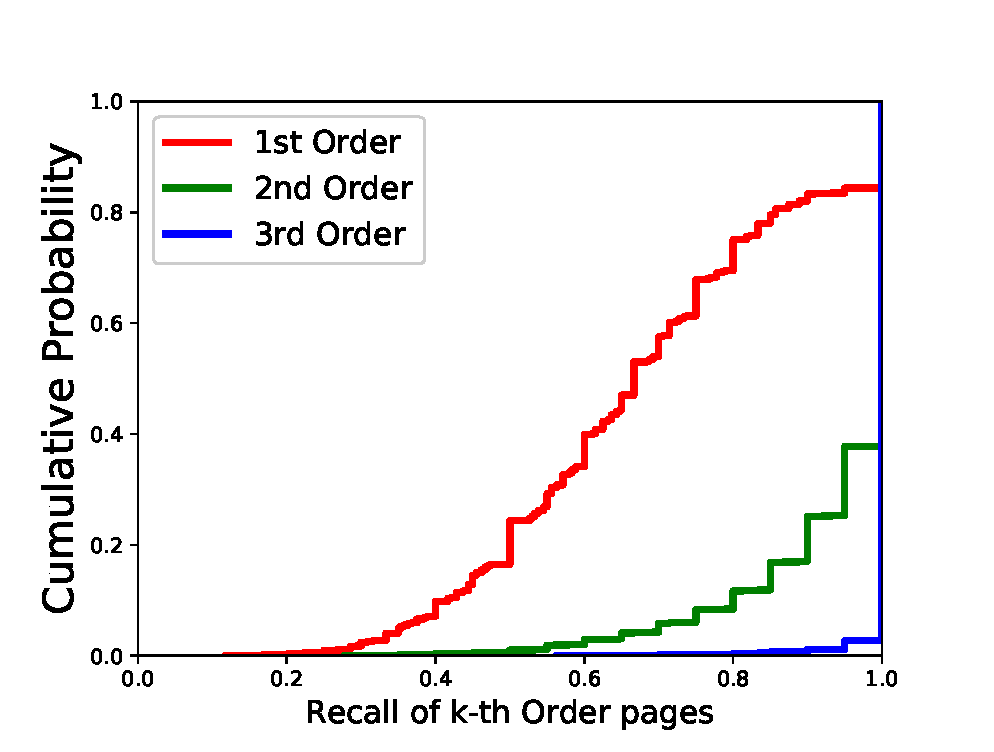
\includegraphics[height=3in]{ratio}
\caption{CFD for $Recall(q,k)$}
\label{fig:cdf}
\end{figure}

As we can see, only in less than $20\%$ of the cases are the top $\sigma(q,1)$ results from WikiNet fully overlap with the first-order pages. In more than $40\%$ of the cases, the top $\sigma(q,1)$ results from WikiNet only contains $60\%$ of the first-order pages. Even when it comes to second-order pages, there are still around $40\%$ of the cases where some of the top $\sigma(q,2)$ (usually 20) results are at least $3$ hops away. 

Another evaluation approach, which foucus on the relationship bewteen the length of the most related path and that of the shortest path may also be feasible. However, since our datasets are extremely biased and limited, we don't think the measurement to be feasible for our datasets. 

\section{Conclusion and futre works}
\label{sec:con}
In this report we presented the project of WikiNet. We implement the prototype based on datasets collected using heuristic methods. We introduce a new document scoring method for networked databases like wikipedia. Results show are WikiNet provide higher-quality information then the na\"ive approach. 

Due to the lack of resource and capability in computation and storage, to stage, the prototype of WikiNet surfers from poor scalibility. It is now working on a single machine, with all data loaded into memory. There is acutally great potential for it to be distributed. 

The traditional vector space model clustering is very computational expensive. 
However, in a networked database, the rich structual information can be used to design a powerful heuristic. 
Remember the fancy visualization of the dataset (Fig.~\ref{fig:net}) ?
The nodes are colored according to the community detection results using the Louvain method \cite{blondel2008fast}. 
The structual based community detection can be carried out immediately after crawling the dataset. 
(At this time, the dataset can only be modeled as a directed yet unweighted graph, but it shouldn't do much damage. ) 
As of 25 April 2017, there are 5,392,540 articles in the English \cite{wikipedia2017size}, the volume of which is a little piece of cake for the Louvain method, and is much computationally cheaper than clustering according to the vector space model. 
A large proportion of the computation and storage was committed to the tf-idf and all-pair most related path. 
For the tf-idf part, at least, it is reasonable to do the computation just within a cluster, because after all, the relations still follows the network structure. Once this idea is veryfiled, the distributing should be intuitive. 

From Section~\ref{sec:eva}, we also get a sense that most of the most related pages are within $3$ clicks from the source. This could also be a reasonable way to design the heuristic. 

Some minor issues of the search engine may be addressed. In this prototype we didn't implement duplication prevention and other search engine architecture optimization technique. From the experiments in Section ~\ref{sec:wikinet}, we know that WikiNet acctually suffer from the lack of these optimizations.  If the project intends to be productionized, these issues should be dealt with. Also, as is indicated in the footnote, our crawler have minor issues to be fixed. 

We canl also spot that there is high degree of overlap between the out-link results and in-link results. We will try merging the results in the future. Query mining is another good way to improve WikiNet. 


\bibliographystyle{abbrv} 
\bibliography{ref}

\end{document}

